\documentclass{article}
\usepackage{graphicx}

\begin{document}
\title{Pictures in LATEX}
\date{}
\maketitle

 Change "Output profile" to LATEX$\Rightarrow$PDF (in drop-down menu). View the PDF output by Adobe Reader \underline{directly from the folder by double-clicking the PDF file} \underline{(not by pressing "view output" in TEXNICCENTER)}.

(Actually one can make Adobe Reader working correctly from TEXNICCENTER in INB2305 by modifying the configuration: in menu "BUILD$\Rightarrow$DEFINE  OUTPUT PROFILES$\Rightarrow$VIEWER" choose profile LATEX$\Rightarrow$PDF in the left pane, then in the three "server" boxes add without space R17 after each "acroview", thus replacing it by "acroviewR17". On the networked machines using PDF is fine, different PDF viewer is linked there.)

\

Top matter should  include \verb#\usepackage{graphicx}#.
Various types of images can be included, here JPG and PDF. The files for the pictures must be either in the same folder as the input file (easiest), or a path should be specified byu a special command in top-matter.


Width and image name are specified in square brackets. Best results as `float' in
figure environment. Then we can refer as ``...see Fig. \ref{pict1}''.

\

\begin{figure}[h] %[h] for `here'
  \centering %optional
  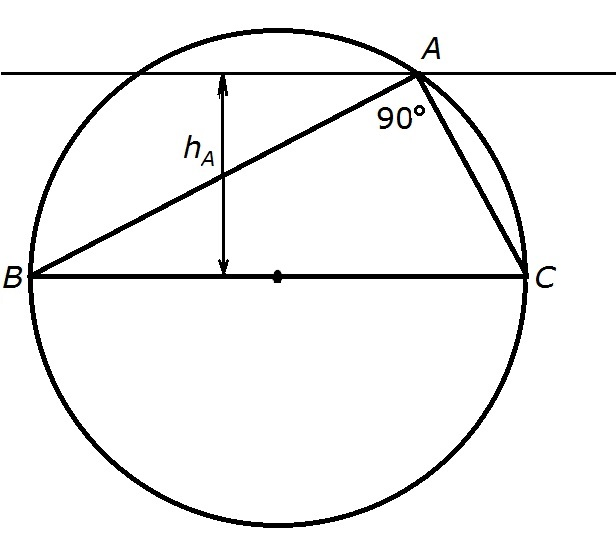
\includegraphics[width=0.2\textwidth]{constr-triangle.jpg}\\ %[width=...] optional
  \caption{How to construct triangle}\label{pict1} %all optional
\end{figure}



\begin{figure}[h]
  \centering
  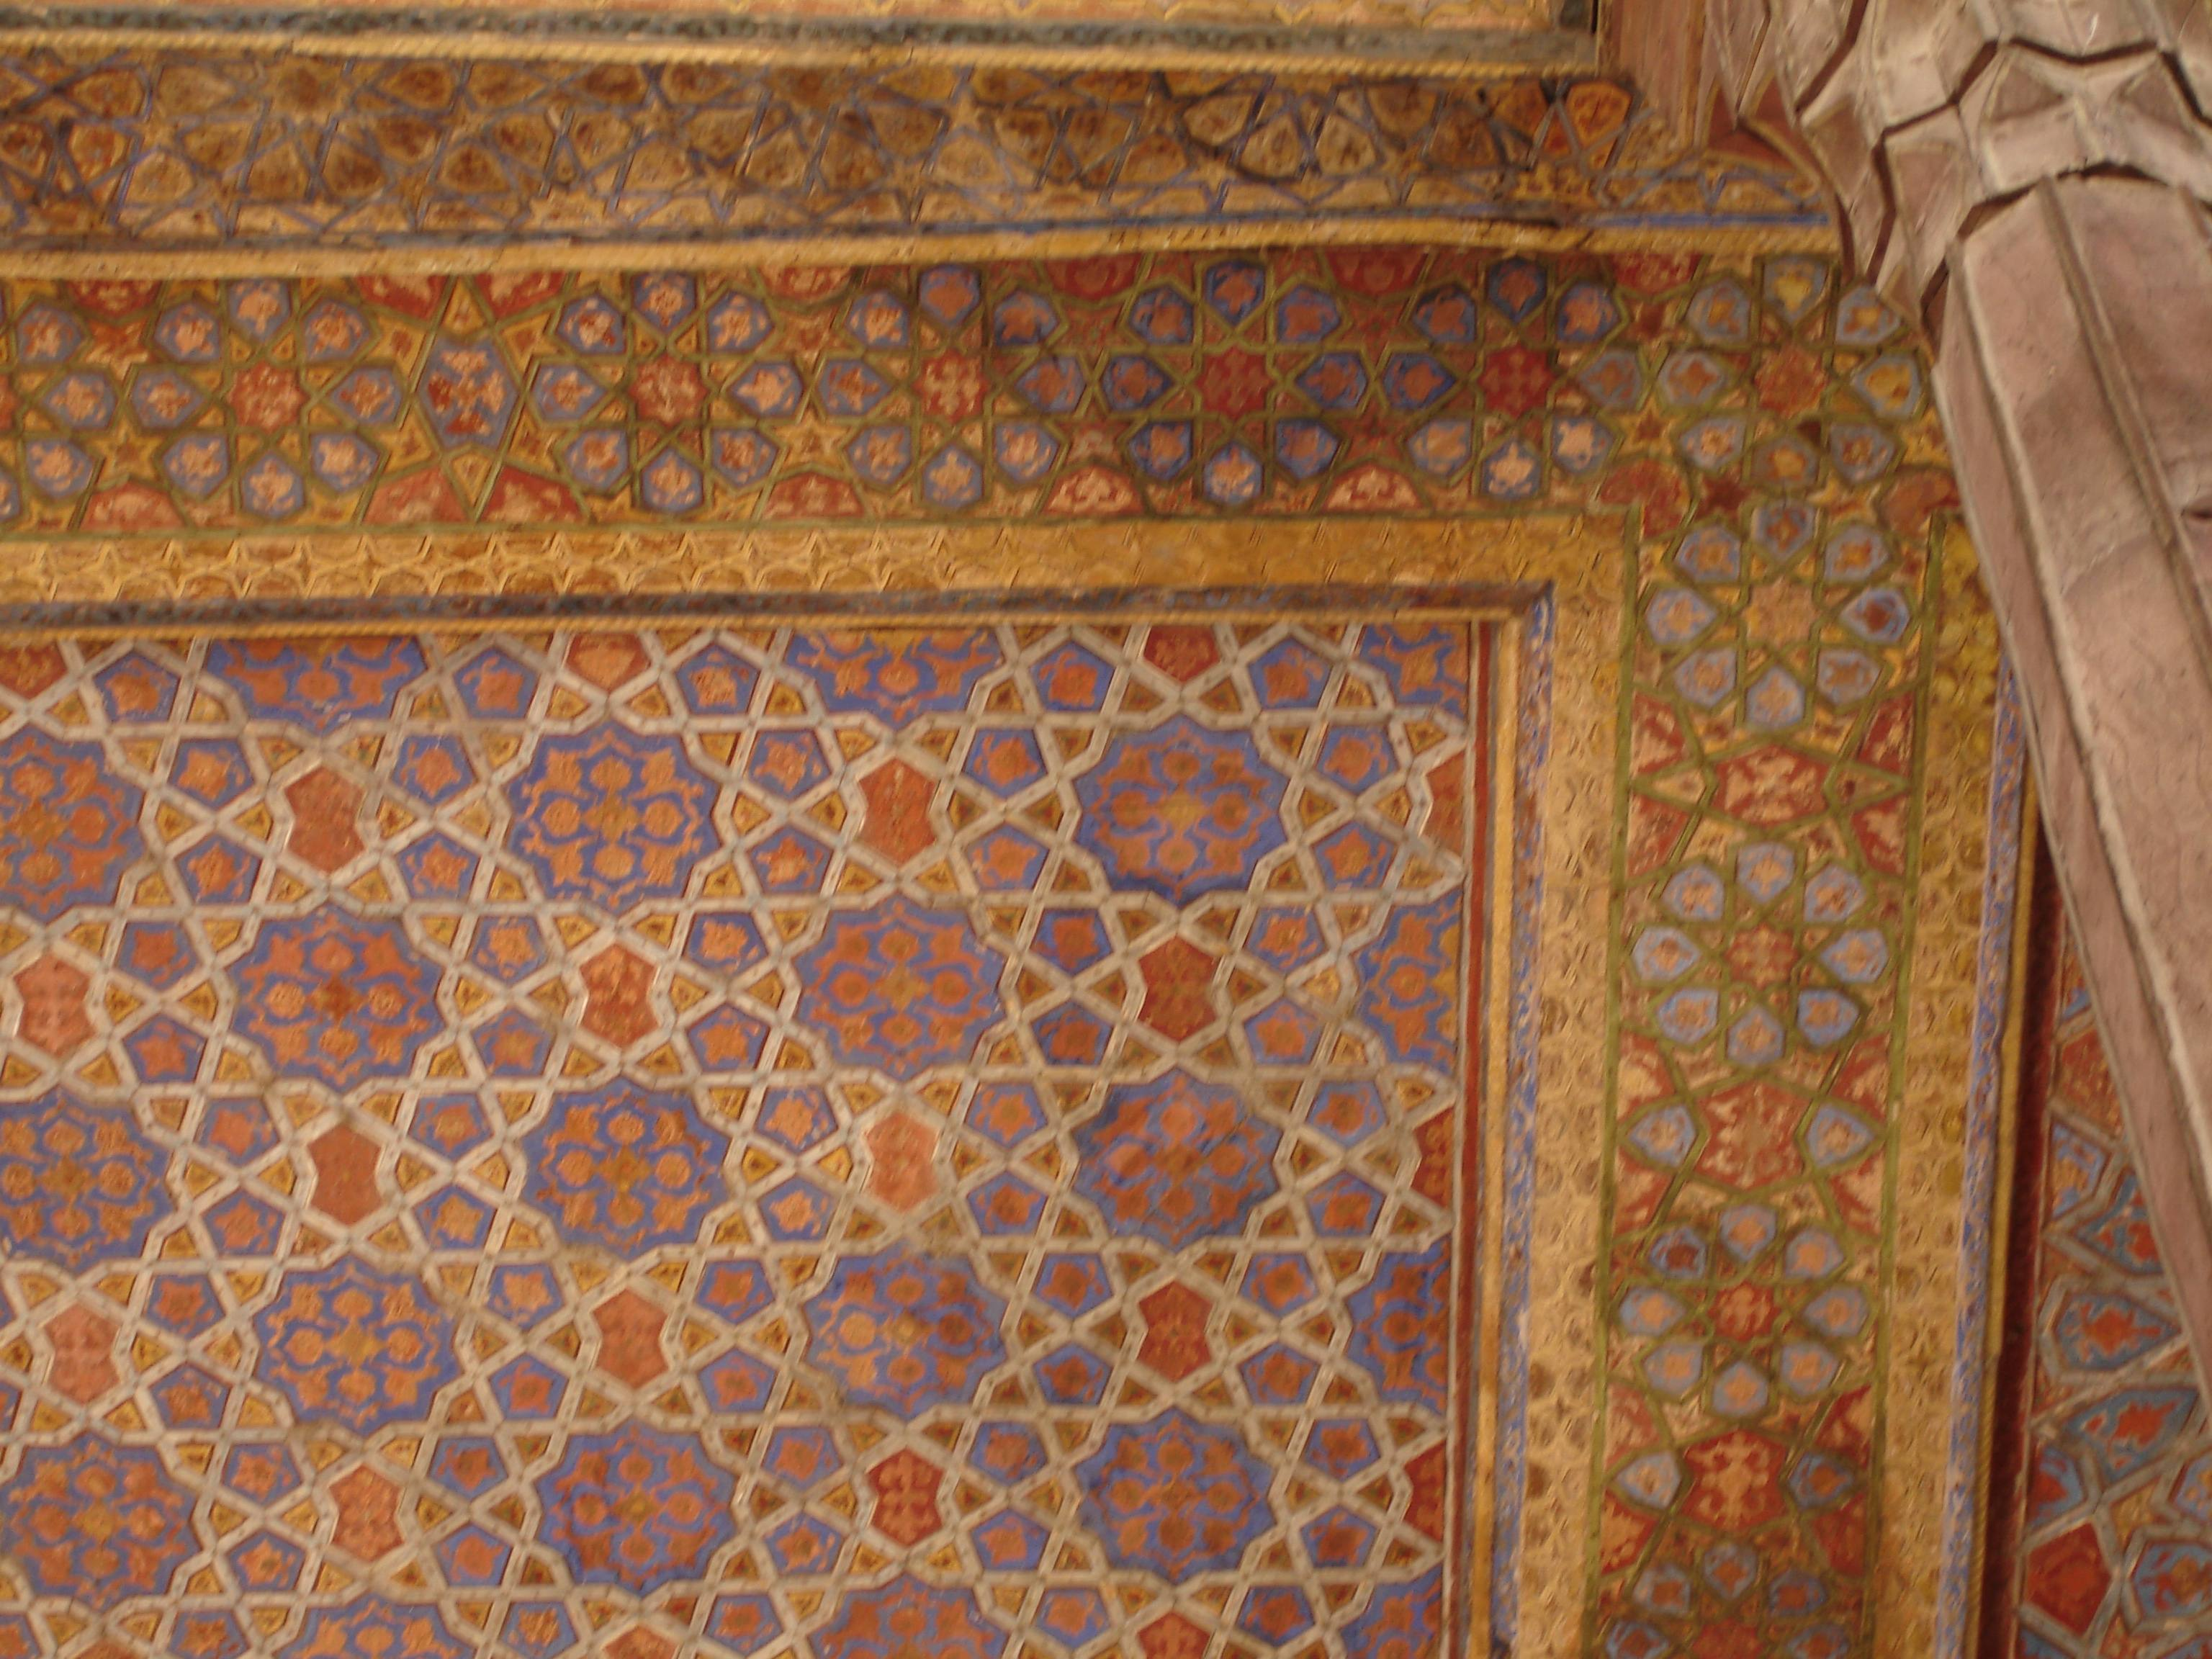
\includegraphics[width=4.5cm]{esf.jpg}\\
  \caption{Ornament with pentagons}\label{orn}
\end{figure}

\begin{figure}[h]
  \centering
  \includegraphics[width=4cm]{map.pdf}\\
  \caption{Campus}\label{map}
\end{figure}


\end{document}            